\section{TensorFlow机制101}
\href{https://www.github.com/tensorflow/tensorflow/blob/r1.4/tensorflow/examples/tutorials/mnist/}{代码}
这个导航的目标是如何使用经典的MNIST数据集用TensorFlow训练和评估前馈神经网络。
\subsection{导航文件}
导航文件如下:
\begin{table}[H]
\centering
	\begin{tabular}{|c|c|}
		\hline
		文件&目的\\
		\hline
		\href{https://www.github.com/tensorflow/tensorflow/blob/r1.4/tensorflow/examples/tutorials/mnist/mnist.py}{mnist.py}&构建完整的全连接的MNIST模型\\
		\hline
		\href{https://www.github.com/tensorflow/tensorflow/blob/r1.4/tensorflow/examples/tutorials/mnist/fully_connected_feed.py}{fully\_connected\_feed.py}&主要代码用来使用feed字典在下载的数据集上训练构建的MNIST模型\\
		\hline 
	\end{tabular}
\end{table}
简单的运行full\_connected\_feed.py文件直接开始训练:\newline
\bashinline{python fully_connected_feed.py}
\subsection{准备数据}
MNIST是一个典型的机器学习问题。这个问题是查看一张$28\times 28$像素的手写数字的灰度图像判断代表0-9中那个值。
\begin{figure}[H]
\centering
\includegraphics[scale=0.5]{mnist_digits.png}
\caption{手写数字'5,0,4,1'}
\end{figure}
更多信息,查看\href{http://yann.lecun.com/exdb/mnist/}{Yann LeCun's MNIST page}或者\href{http://colah.github.io/posts/2014-10-Visualizing-MNIST/}{Chris Olah's visualizations of MNIST}。
\subsection{下载}
在run\_training()方法前,input\_data.read\_data\_sets()函数将确保正确的数据下载到了你的本地训练文件夹然后解压数据返回一个Dataset实例字典。
\pythoninline{data_sets = input_data.read_data_sets(FLAGS.train_dir, FLAGS.fake_data)}
注意:fake\_data 标志用于单位测试意图可以被忽略。
\begin{table}[H]
\centering
	\begin{tabular}{|c|c|}
	\hline 
		数据集&目的\\
		\hline
		data\_sets.train&55000图像和标签,用于训练\\
		\hline
		data\_set.validation&5000图像和标签用于交叉验证训练精度\\
		\hline
		data\_sets.test&10000图像和标签,用于测试训练精度\\
	\end{tabular}
\end{table}
\subsection{输入和Placeholder}
一个placeholder\_inputs()函数创建两个\href{https://www.tensorflow.org/api_docs/python/tf/placeholder}{tf.placeholder}操作定义输入形状,包含batch\_size,重置图进入实际训练。
\begin{pythoncode}
images_placeholder = tf.placeholder(tf.float32, shape=(batch_size,
                                                       mnist.IMAGE_PIXELS))
labels_placeholder = tf.placeholder(tf.int32, shape=(batch_size))
\end{pythoncode}
在循环中,完整的图像和标签数据集被切片为每步适合batch\_size,匹配placeholder操作,然后使用feed\_dict参数传递进sess.run()。
\subsection{构建图}
在为数据创建placeholder的时候,图是从mnist.py文件根据三个模块构建的。
\begin{enumerate}
\item inference()构建图运行网络预测
\item loss()添加推理图操作要求生成损失
\item training()添加损失图操作要求计算和应用梯度
\end{enumerate}
\begin{figure}[H]
\centering
\includegraphics[scale=0.5]{mnist_subgraph.png}
\caption{TensorBoard框架}
\end{figure}
\subsection{推理}
inference()函数构建图返回预测输出。它接受图像placeholder作为输入构建在全连接的顶部结合10节点的先形层指定ReLU激活。
每个曾在tf.name\_scope创建作为一个创建scope的前缀:\pythoninline{with tf.name_scope('hidden1'):}

在定义的scope中,权重和偏执被每层使用生成希望的tf.Variable实例:
\begin{pythoncode}
weights = tf.Variable(
    tf.truncated_normal([IMAGE_PIXELS, hidden1_units],
                        stddev=1.0 / math.sqrt(float(IMAGE_PIXELS))),
    name='weights')
biases = tf.Variable(tf.zeros([hidden1_units]),
                     name='biases')
\end{pythoncode}
对于实例在hidden1 scope下创建,将给权重独特的名字"hidden1/weights"。

每个变量给定初始化的操作作为他们构造的一部分。在这制表符情况下,权重被tf.truncated\_normal初始化,给定第一维代表权重连接的层数,第二维度表示权重连接的单元2-D tensor。对第一层,命名为hidden1,维度[IMAGE\_PIXELS,hidden1\_units]因为权重连接图像输入到hidden1层。tf.truncated\_normal初始化根据给定的均值和标准差生成正态分布。

然后偏执被初始化tf.zeros确保他们用所有的0值开始,然后他们的形状是这层简单的单元数量。

图有三个主要操作,两个tf.nn.relu操作为隐藏层和额外的tf.atmul包装tf.matmul,然后创建分开tf.Variable实例连接输入placeholder或者之前层的输出tensor。
\begin{pythoncode}
hidden1 = tf.nn.relu(tf.matmul(images, weights) + biases)
hidden2 = tf.nn.relu(tf.matmul(hidden1, weights) + biases)
logits = tf.matmul(hidden2, weights) + biases 
\end{pythoncode}
最后,logits tensor将包含的输出返回。
\subsection{损失}
loss()函数通过添加损失操作进一步构建图。
首先labels\_placeholder转化为64位的整数。然后一个tf.nn.sparse\_softmax\_cross\_entropy\_with\_logits操作被添加自动从labels\_placeholder生成1-hot标签和比较inference的1-hot标签的输出logits。
\begin{pythoncode}
abels = tf.to_int64(labels)
lcross_entropy = tf.nn.sparse_softmax_cross_entropy_with_logits(
    labels=labels, logits=logits, name='xentropy')
\end{pythoncode}
它使用tf.reduce\_mean平均batch维度上的交叉熵值作为总损失。\newline 
\pythoninline{loss = tf.reduce_mean(cross_entropy,name='xentropy_mean')}
tensor将包含返回的损失值。
\subsection{训练}
training()函数添加需要的操作通过梯度下降最小化损失。首先,它接受loss()函数的损失tensor处理它为一个\href{https://www.tensorflow.org/api_docs/python/tf/summary/scalar}{tf.summary.scalar},一个操作使用\href{https://www.tensorflow.org/api_docs/python/tf/summary/FileWriter}{tf.summary.FileWriter}生成总结的值到事件文件。在这种情况下损失每个时间的值被发送给总结写入事件文件。
\pythoninline{tf.summary.scalar('loss', loss)}

下一步我们实例化\href{https://www.tensorflow.org/api_docs/python/tf/train/GradientDescentOptimizer}{tf.train.GradientDescentOptimizer }表达,结合学习率应用梯度。\newline
\pythoninline{optimizer = tf.train.GradientDescentOptimizer(learning_rate)}
我们生辰给一个单一变量包含全局训练步数和\href{https://www.tensorflow.org/api_docs/python/tf/train/Optimizer#minimize}{tf.train.Optimizer.minimize }操作用于更新系统中可训练的权重增加全局不是。op正如train\_op必须通过一个TensorFlow会话减少训练的完整步数(如下)。
\begin{pythoncode}
global_step = tf.Variable(0, name='global_step', trainable=False)
train_op = optimizer.minimize(loss, global_step=global_step)
\end{pythoncode}
\subsection{训练模型}
当图被构建的时候,他可以通过在fully\_connected\_feed.py中的代码在循环中交互式的训练和评估。
\subsection{图}
run\_training()函数的顶端是一个with命令预示所有的构建操作被默认的全局\href{https://www.tensorflow.org/api_docs/python/tf/Graph}{tf.Graph }图结合。可以使用更复杂的多图,但是超过了这个导航的范围。
\subsection{会话}
当构建操作被完全添加所有的需要的操作被生成,一个\href{https://www.tensorflow.org/api_docs/python/tf/Session}{tf.Session}为了运行图被创建。
\pythoninline{sess = tf.Session()}
一个Session可与在with块中生成:\pythoninline{with tf.Session() as sess:}
这个session空的参数预示着代码将添加默认的本地图。在创建会话后,所有的tf.Variable实例通过在初始化操作上的\href{https://www.tensorflow.org/api_docs/python/tf/Session#run}{tf.Session.run}初始化。
\begin{pythoncode}
init = tf.global_variables_initializer()
sess.run(init)
\end{pythoncode}
tf.Session.run方法将运行子图,对应的操作将操作参数传入。在第一次调用的时候init操作包含初始化的变量。没有重置的图在这里运行,发生在下面的训练循环中。
\subsection{训练循换}
在结合会话初始化变量后,训练也许开始。用户的代码控制训练的步数,最简单的循环可以训练的时候很有用:
\begin{pythoncode}
for step in range(FLAGS.max_steps):
    sess.run(train_op)
\end{pythoncode}
然而,这个导航有一点复杂在这里必须为每步slice up输入数据匹配先前的placeholder。
\subsection{feed图}
对于每一步,代码将生成一个包含一些样本的feed字典训练。在fill\_feed\_dict()函数中,给定的DatSet要求图像和标签的,tensor匹配placeholder被包含下一批的图像和标签填充一个batch\_size。
\begin{pythoncode}
images_feed, labels_feed = data_set.next_batch(FLAGS.batch_size,
                                               FLAGS.fake_data)
\end{pythoncode}
一个Python字典对象被placeholder作为key作为值表示feed tensor。
\begin{pythoncode}
feed_dict = {
    images_placeholder: images_feed,
    labels_placeholder: labels_feed,
}
\end{pythoncode}
这传递sess.run()函数的feed\_dict参数在训练过程中提供输入样本。
\subsection{检查状态}
代码指定两个值在run调用的时候获取数据:[train\_op,loss]
\begin{pythoncode}
for step in xrange(FLAGS.max_steps):
    feed_dict = fill_feed_dict(data_sets.train,
                               images_placeholder,
                               labels_placeholder)
    _, loss_value = sess.run([train_op, loss],
                             feed_dict=feed_dict)
\end{pythoncode}
因为有两个值要获取,sess.run()返回一个两个元素的元祖。每个列表中的Tensor在返回的tuple中获取numpy数组值,在训练中填充tensor的值。因此train\_op是一个没有输出值的操作,对应的元素在返回的元祖中为None,被丢弃。然而,如果模型在训练中loss Tensor的值也许变为NaN,因此我们捕获这个值用于logging。

假设训练没有NaN也能返回,训练循环每100步打印一个简单的状态让使用者知道训练的状态。
\begin{pythoncode}
if step % 100 == 0:
    print('Step %d: loss = %.2f (%.3f sec)' % (step, loss_value, duration))
\end{pythoncode}
\subsection{可视化状态}
为了发送TensorBoard生成的事件文件,所有的总结在图构建起见被收集进一个Tensor。
\pythoninline{summary = tf.summary.merge_all()}
会话被创建后,一个\href{https://www.tensorflow.org/api_docs/python/tf/summary/FileWriter}{tf.summary.FileWriter}被实例化写包含图本身和总结值的事件文件。
\pythoninline{summary_writer = tf.summary.FileWriter(FLAGS.train_dir, sess.graph)}

最后,事件每次文件被新的总结值更新被评估和输出writer的add\_summary()函数。
\begin{pythoncode}
summary_str = sess.run(summary, feed_dict=feed_dict)
summary_writer.add_summary(summary_str, step)
\end{pythoncode}
当事件文件被写后,TensorBoard也许被再次运行从总结文件中显示值:
\begin{figure}[H]
\centering
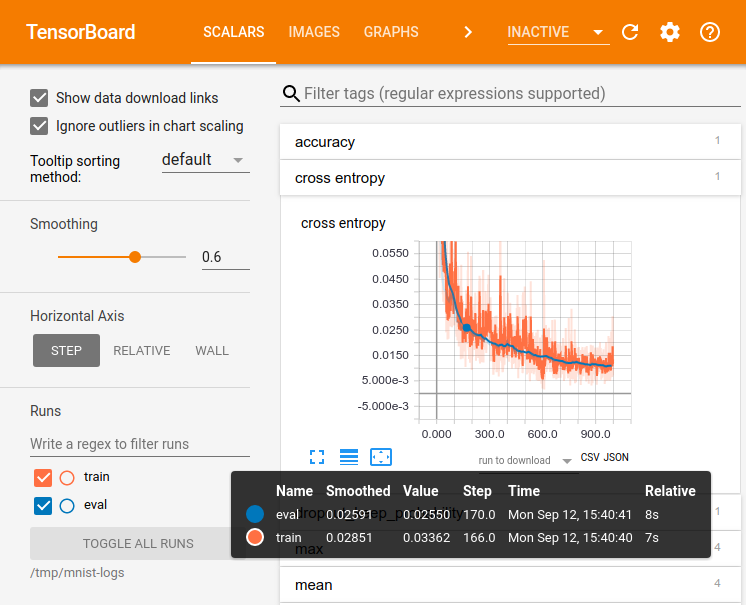
\includegraphics[scale=0.5]{mnist_tensorboard.png}
\caption{TensorBoard}
\end{figure}
\subsection{保存一个Checkpoint}
为了发送一个用于进一步训练和评估的checkpoint文件,我们实例化\href{https://www.tensorflow.org/api_docs/python/tf/train/Saver}{tf.train.Saver}。
\pythoninline{saver = tf.train.Saver()}
为了训练循换\href{https://www.tensorflow.org/api_docs/python/tf/train/Saver#save}{tf.train.Saver.save}方法将周期性被调用通过结合当前可训练的变量的值写入一个checkpoint文件进训练目录。\pythoninline{saver.save(sess, FLAGS.train_dir, global_step=step)}。
在之后一些更新的点,训练也许被通过\href{https://www.tensorflow.org/api_docs/python/tf/train/Saver#restore}{tftrain.Saver.restore}方法重载模型参数。\newline
\pythoninline{saver.restore(sess, FLAGS.train_dir)}

\subsection{评估模型}
每1000步,代码将尝试在训练和测试集上评估模型。do\_eval()函数被调用三次,用于训练,验证和测试集。
\begin{pythoncode}
print('Training Data Eval:')
do_eval(sess,
        eval_correct,
        images_placeholder,
        labels_placeholder,
        data_sets.train)
print('Validation Data Eval:')
do_eval(sess,
        eval_correct,
        images_placeholder,
        labels_placeholder,
        data_sets.validation)
print('Test Data Eval:')
do_eval(sess,
        eval_correct,
        images_placeholder,
        labels_placeholder,
        data_sets.test)

\end{pythoncode}
注意更多的复杂用法将通常隔绝data\_sets.test仅仅在重要的参数调整后被检查。为了一个简单的MNIST问题,我们评估所有的数据。
\subsection{构建评估图}
在输入训练循环之前,Eval操作应该被mnist.py中的evaluation()结合logits/labels参数作为损失函数构建。\newline
\pythoninline{eval_correct = mnist.evaluation(logits, labels_placeholder)}\newline
evaluation()函数简单的生成一个\href{https://www.tensorflow.org/api_docs/python/tf/nn/in_top_k}{tf.nn.in\_top\_k}操作可以自动的对每个模型输出评分。在这种情况下,我们仅仅考虑如果label为True是k设置为1。\newline
\pythoninline{eval_correct = tf.nn.in_top_k(logits, labels, 1)}
\subsection{评估输出}
可以创建一个训练填充feed\_dict调用sess.run()eval\_correct操作在给定的数据集上评估模型:
\begin{pythoncode}
for step in range(steps_per_epoch):
    feed_dict = fill_feed_dict(data_set,
                               images_placeholder,
                               labels_placeholder)
    true_count += sess.run(eval_correct, feed_dict=feed_dict)
\end{pythoncode}
true\_count变量简单的求和所有的预测in\_top\_k操作决定正确预测。精度可以通过除以总共统计的样本数求得。
\begin{pythoncode}
precision = true_count / num_examples
print('  Num examples: %d  Num correct: %d  Precision @ 1: %0.04f' %
      (num_examples, true_count, precision))
\end{pythoncode}
